\documentclass[dvipsnames]{beamer}
\mode<presentation>{}
\usepackage[utf8]{inputenc}
\usepackage{amsmath, amssymb, amsfonts, amsthm, mathtools, mathrsfs}
\setbeamertemplate{theorems}[numbered]
\title{\texorpdfstring{$\mathbb{C}$}{C}omplex Analysis TSC}
\author[Aryaman Maithani]{\texorpdfstring{Aryaman Maithani\\\url{https://aryamanmaithani.github.io/tuts/ma-205}}{Aryaman Maithani}}
\date{Autumn Semester {\color{red}2020}-21}
\institute[IITB]{IIT Bombay}
\usetheme{Warsaw}
% \usecolortheme{beetle}
\hypersetup{colorlinks=true}
\addtobeamertemplate{footline}{\hypersetup{allcolors=.}}{}
\usepackage{parskip}
\usepackage{tcolorbox}

\usepackage{tikz}
\usetikzlibrary{decorations.markings}
\usetikzlibrary{arrows.meta}

\newcommand{\id}{\operatorname{id}}
\newcommand{\Res}{\operatorname{Res}}
% \renewcommand{\exp}{\operatorname{exp}}

\theoremstyle{definition}
\newtheorem{defn}{Definition}
\newtheorem{prop}{Proposition}
\newtheorem{thm}{Theorem}
\newtheorem{rem}{Remark}

\begin{document}
\tikzset{lab dis/.store in=\LabDis,
  lab dis=-0.4,
  ->-/.style args={at #1 with label #2}{decoration={
    markings,
    mark=at position #1 with {\arrow{>}; \node at (0,\LabDis) {#2};}},postaction={decorate}},
  -<-/.style args={at #1 with label #2}{decoration={
    markings,
    mark=at position #1 with {\arrow{<}; \node at (0,\LabDis)
    {#2};}},postaction={decorate}},
  -*-/.style args={at #1 with label #2}{decoration={
    markings,
    mark=at position #1 with {{\fill (0,0) circle (1.5pt);} \node at (0,\LabDis)
    {#2};}},postaction={decorate}},
  }
\begin{frame}
    \titlepage
\end{frame}
\begin{frame}{Greetings}
    Hi, \uncover<2->{welcome to this }
    \begin{center}
        \uncover<3->{\emph{complex}} \uncover<4->{discussion. }
    \end{center}
    \uncover<5->{Here are some ``guidelines'' for this TSC - }
    \begin{enumerate}
        \uncover<6->{\item Unmute your mic at any time and ask your doubt. }
        \uncover<7->{\item I will not be checking chat often (or maybe at all), so posting it there might not be helpful. }
    \end{enumerate}
    \uncover<8->{You can find a link to this document on \url{bit.ly/ca-205}. Both with and without pauses. You may keep it open alongside for quick reference. }
\end{frame}
\begin{frame}{Warning}
    This is primarily going to be a quick recap of the facts important.\\
    \uncover<2->{It is, of course, not possible to go through everything in just 2 hours. }\\
    \uncover<3->{In particular, this will \emph{not} be a substitute for all the lectures done so far. }\\
    \uncover<4->{I will also not be going through the proofs. }\uncover<5->{We can discuss these finer things at the end, if time permits. }\\
    \uncover<6->{Though I'm not a fan of this - this session is pretty much going to cover things important from the point of view of an exam. }\uncover<7->{I may also skip things from the lectures if I think that they are not important. }\uncover<8->{They \emph{might} turn out to be important, though. }

    \uncover<9->{Of course, I will not \uncover<10->{(intentionally)} say anything which is mathematically incorrect. }
\end{frame}
\begin{frame}{Lecture 1}
    \begin{defn}[Some notation]
        Given $z_0 \in \mathbb{C}$ and $\delta > 0,$ the $\delta$-neighbourhood of $z_0,$ denoted by $B_\delta(z_0)$ is the set
        \begin{equation*} 
            B_\delta(z_0) \vcentcolon= \{z \in \mathbb{C} : |z - z_0| < \delta\}.
        \end{equation*}
    \end{defn}
    \uncover<2->{\begin{defn}[Open sets]
            A set $U \subset \mathbb{C}$ is said to be open if:\\
            for \emph{every} $z_0 \in \mathbb{C},$ there exists \emph{some} $\delta > 0$ such that
            \begin{equation*} 
                B_\delta(z_0) \subset U.
            \end{equation*}
        \end{defn} }
    \uncover<3->{\begin{defn}[Path-connected sets]
        A set $P \subset \mathbb{C}$ is said to be path-connected if any two points in $P$ can be joined by a path in $P$. (A continuous function from $[0, 1]$ to $P.$)
    \end{defn} }
    % \uncover<4->{Examples and more? There in slides as well as the informal-tut that I took on 21st August {\color{red}2020}.}
\end{frame}
\begin{frame}{Lecture 1}
    \begin{defn}[Differentiable]
        Let $\Omega \subset \mathbb{C}$ be {\color<2->{red}{open}}. Let
        \begin{equation*} 
            f:\Omega \to \mathbb{C}
        \end{equation*}
        be a function. \uncover<3->{Let $z_0 \in \Omega.$ }\uncover<4->{$f$ is said to be \emph{differentiable} at $z_0$ if }
        \uncover<5->{
        \begin{equation*} 
            \lim_{z\to z_0}\dfrac{f(z) - f(z_0)}{z - z_0}
        \end{equation*} }
        \uncover<6->{exists. In this case, it is denoted by $f'(z_0).$}
    \end{defn}
\end{frame}
\begin{frame}{Lecture 1}
    \begin{defn}[Holomorphic]
        A function $f$ is said to be holomorphic on an open set $\Omega$ if it is differentiable at every $z_0 \in \Omega.$

        A function $f$ is said to be holomorphic at $z_0$ if it is holomorphic on some neighbourhood of $z_0.$
    \end{defn}
    \uncover<2->{\begin{rem}
        A function may be differentiable at $z_0$ but not holomorphic at $z_0$. \\
        \uncover<3->{For example, $f(z) = |z|^2$ is differentiable only at $0.$ }\uncover<4->{Thus, it is differentiable at $0$ but holomorphic nowhere. }
    \end{rem} }
    \uncover<5->{For sets, however, there is no difference. }
\end{frame}
\begin{frame}{End of Lecture 1}
    \begin{tcolorbox}
        Any questions?
    \end{tcolorbox}
\end{frame}
\begin{frame}{Notation}
    From this point on, $\Omega$ be always denote an open subset of $\mathbb{C}.$\\
    Whenever I write some complex number $z$ as $z = x + \iota y,$ it will be assumed that $x, y \in \mathbb{R}.$\\
    Similarly for $f(z) = u(z) + \iota v(z).$
\end{frame}
\begin{frame}{Lecture 2: CR Equations}
    Let $f:\Omega \to \mathbb{C}$ be a function. We can decompose $f$ as
    \begin{equation*} 
        f(z) = u(z) + \iota v(z),
    \end{equation*}
    where $u, v : \Omega \to \mathbb{R}$ are real valued functions.

    \uncover<2->{The idea now is to consider $u$ and $v$ as functions of two variables. We can do so by simply considering $u(x, y) = u(x + \iota y)$ and similarly for $v.$ }
    \uncover<3->{Now, if we know that $f$ is holomorphic, then we have the following result. }
\end{frame}
    
\begin{frame}{Lecture 2: CR Equations}
    \uncover<1->{\begin{thm}[CR equations]
        Let $f:\Omega\to\mathbb{C}$ be differentiable at {\color{red}a point} $z_0 \in \Omega.$ Let $z_0 = x_0 + \iota y_0.$\\
        \uncover<2->{Then, we have
                \begin{equation*} 
                    u_x(x_0, y_0) = v_y(x_0, y_0) \quad\text{and}\quad u_y(x_0, y_0) = -v_x(x_0, y_0). }
        \end{equation*}
        \uncover<3->{Moreover, we have
        \begin{equation*} 
            f'(z_0) = u_x(x_0, y_0) + \iota v_x(x_0, y_0). 
        \end{equation*}
        \uncover<4->{Existence of $u_x, u_y, v_x, v_y$ is part of the theorem. } }
    \end{thm} }
    \uncover<5->{Note the subscript is $x$ for both in the above. }\\
    \uncover<6->{Also note that all the equalities are only at {\color{red}the point $z_0.$} }\uncover<7->{In particular, we are only assuming differentiability at $z_0.$ }
\end{frame}
\begin{frame}{Lecture 2: CR Equations}
    Converse? What is the converse? Is it true? 

    \uncover<2->{{\color{red}No.} The converse is {\color{red}not} true. }

    \uncover<3->{An example for you to check is
    \begin{equation*} 
        f(z) \vcentcolon= \begin{cases}
            \dfrac{\bar{z}^2}{z} & z \neq 0,\\
            0 & z = 0.
        \end{cases}
    \end{equation*} }\uncover<4->{Check that $u$ and $v$ satisfy the CR equations at $(0, 0)$ but $f$ is not differentiable at $0 + 0\iota.$ (Page 23 of slides.)}
\end{frame} 
\begin{frame}{Lecture 2: CR Equations}
    We recall MA 105 now.  
    \begin{defn}[Total derivative] 
    If $f:\Omega\to\mathbb{C}$ is a function, we may view it as a function
    \begin{equation*} 
        f:\Omega\to\mathbb{R}^2.
    \end{equation*}
    Recall that $f$ is said to be real differentiable at $(x_0, y_0) \in \Omega \subset \mathbb{R}^2$ if \uncover<2->{there exits a $2\times2$ real matrix $A$ such that }
    \uncover<3->{\begin{equation*} 
            \lim_{(h, k)\to (0, 0)}\dfrac{\left\|f(x_0 + h, y_0 + k) - f(x_0, y_0) - A\begin{bmatrix}
                h\\
                k
            \end{bmatrix}\right\|}{\|(h, k)\|} = 0.
        \end{equation*} }
    \uncover<4->{The matrix $A$ was called the \emph{total derivative of $f$ at $(x_0, y_0)$.} }
    \end{defn}
\end{frame}
\begin{frame}{Lecture 2: CR Equations}
    \begin{thm}[]
        If $f$ is (complex) differentiable at {\color{red}a point} $z_0 = x_0 + \iota y_0,$ then $f$ is real differentiable at $(x_0, y_0).$
    \end{thm}
    \uncover<2->{Once again, this is only talking about differentiability at a point. }\\
    \uncover<3->{The converse is again {\color{red}not} true. }\\
    \uncover<4->{Take the example $f(z) = \bar{z}.$ }
    \uncover<5->{Thus, we have seen two sufficient conditions for complex differentiability so far. Neither is individually sufficient. }\uncover<6->{However, together, they are. }
\end{frame}
\begin{frame}{Lecture 2: CR Equations}
    \begin{thm}[]
        Let $f:\Omega\to\mathbb{C}$ be a function and let $z_0 = x_0 + \iota y_0 \in \Omega.$ If \\
        \uncover<2->{the CR equations hold {\color{red}at the point} $(x_0, y_0)$ and \\ }
        \uncover<3->{if $f$ is real differentiable {\color{red}at the point} $(x_0, y_0),$ then \\ }
        \uncover<4->{$f$ is complex differentiable {\color{red}at the point} $z_0.$ }
    \end{thm}
\end{frame}
\begin{frame}{Lecture 2: CR Equations}
    \begin{defn}[Harmonic functions]
        Let $u:\Omega\to\mathbb{R}^2$ be a twice continuously differentiable function. $u$ is said to be \emph{harmonic} if $u_{xx} + u_{yy} = 0.$
    \end{defn}
    \uncover<2->{\begin{prop}[]
            The real and imaginary parts of a holomorphic function are harmonic.
        \end{prop} }
    \uncover<3->{Suppose $u$ and $v$ are harmonic on $\Omega.$ $v$ is said to be {\color{red}a} harmonic conjugate of $u$ if $f = u + \iota v$ is holomorphic on $\Omega.$ }\\
    \uncover<4->{If $v$ is a harmonic conjugate of $u,$ then $-u$ is a harmonic conjugate of $v.$ }\\
    \uncover<5->{Check the second last slide of this lecture to find the algorithm for finding a harmonic conjugate. }
\end{frame}
\begin{frame}{End of Lecture 2}
    \begin{tcolorbox}
        Any questions?
    \end{tcolorbox}
\end{frame}
\begin{frame}{Lecture 3: Power Series}
    \begin{defn}[Convergence of series]
        A series of the form 
        \begin{equation*} 
            \sum_{n = 0}^{\infty}a_n
        \end{equation*}
        of complex numbers is said to converge if the sequence of partial sums
        \begin{equation*} 
            s_n = \sum_{k = 0}^{n}a_k
        \end{equation*}
        converges (to a finite complex number).
    \end{defn}
    \uncover<2->{The sequence of partial sums is just the following sequence:
    \begin{equation*} 
        a_0, a_0 + a_1, a_0 + a_1 + a_2, \ldots.
    \end{equation*} }
    \uncover<3->{``Divergent'' is simply used to mean ``not convergent.'' }\\
    \uncover<4->{Check that $\sum_{}^{}(-1)^n$ and $\sum_{}^{}n$ both diverge. }
\end{frame}
\begin{frame}{Lecture 3: Power Series}
    \begin{defn}[limsup]
        Given a sequence $(x_n)$ of {\color{red}real numbers}, we may define a new sequence $(y_n)$ as\uncover<2->{
        \begin{equation*} 
            y_n = \sup\{x_m : m \ge n\}.
        \end{equation*} }
        \uncover<3->{The limit of this sequence always exists and we define
        \begin{equation*} 
            \limsup_{n\to\infty}x_n = \lim_{n\to\infty}y_n.
        \end{equation*} }
    \end{defn}
    \uncover<4->{\begin{rem}
        Each $y_n$ might be $\infty.$ That is allowed.\\
        \uncover<5->{The limsup might be $\pm\infty.$ This is also allowed. }\\
        \uncover<6->{If $\displaystyle\lim_{n\to \infty}x_n$ itself exists, then it equals the $\limsup$ as well. }
    \end{rem} }
\end{frame}
\begin{frame}{Lecture 3: Power Series}
    We will be interested in discussing radius of convergence of \emph{power series.} We all know what that is. It is a series of the form
    \begin{equation*} 
        \qquad \sum_{n = 0}^{\infty}a_n(z - z_0)^n \qquad {\color{ForestGreen}{(*)}}
    \end{equation*}
    where $z_0 \in \mathbb{C}$ and each $a_n \in \mathbb{C}.$

    \uncover<2->{What is the radius of convergence, though? }\uncover<3->{(The definition, that is.) }\\
    \uncover<3->{\begin{thm}[Radius of convergence]
        Given any power series as ${\color{ForestGreen}{(*)}},$ there exists $R \in {\color<5->{red}{[}}0, \infty{\color<5->{red}{]}}$ such that
        \begin{enumerate}
            \item {\color{ForestGreen}{$(*)$}} converges for any $z$ with $|z - z_0| < R$\uncover<4->{, and
            \item {\color{ForestGreen}{$(*)$}} diverges for any $z$ with $|z - z_0| > R.$ }    
        \end{enumerate}
        This $R$ is called the radius of convergence.
    \end{thm} }
    \uncover<5->{Note the {\color{red}brackets}. }
\end{frame}
\begin{frame}{Lecture 3: Power Series}
    We would now like to be able to calculate the radius of convergence.
    \begin{thm}[Root test]
        \uncover<2->{Let {\color{ForestGreen}{$(*)$}} be as earlier. Define
        \begin{equation*} 
            \alpha = \limsup_{n \to \infty}\sqrt[n]{\left|a_n\right|}.
        \end{equation*} }
        \uncover<3->{Then, $R = \alpha{\color{red}^{-1}}$ is the radius of convergence. }
    \end{thm}
    \uncover<4->{This test \emph{always works.} We had no assumptions of any kind on ${\color{ForestGreen}{(*)}}.$ }\\
    \uncover<5->{Note that {\color{red}$^{-1}$}. }\\
    \uncover<6->{If $\alpha = 0,$ then $R = \infty$ and vice-versa. }
\end{frame}
\begin{frame}{Lecture 3: Power Series}
    We have another test. This is simpler (to calculate) but mightn't always work.
    \begin{thm}[Ratio test]
        Let {\color{ForestGreen}{$(*)$}} be as earlier.\\
        \uncover<2->{{\color{red}Assume that} the limit 
        \begin{equation*} 
            R = \lim_{n\to \infty} \left|\dfrac{a_{\color{red}n}}{a_{{\color{red}n+1}}}\right|
        \end{equation*} 
        exists. (Possibly as $\infty.$)}\\
        \uncover<3->{Then, $R$ is the radius of convergence. }
    \end{thm}
    \uncover<4->{Note that here we assume that the limit does exist. This may not always be true. }\\
    \uncover<5->{Note that I'm not taking any inverse here but also note the way the ratio is taken. We have $a_n/a_{n+1}.$ }
\end{frame}
\begin{frame}{Lecture 3: Power Series}
    Differentiability of power series is what one should expect.
    \begin{thm}[Differentiability]
        Let $\sum_{n = 0}^{\infty}a_nz^n$ be a power series with radius of convergence $R > 0.$ On the {\color{red}open disc} of radius $R,$ let $f(z)$ denote this sum. Then, on this disc, we have
        \begin{equation*} 
            f'(z) = \uncover<2->{\sum_{n = 1}^{\infty}na_nz^{n-1}.}
        \end{equation*}
    \end{thm}
    \uncover<3->{Note that this is again a power series with the same radius of convergence. Thus, we may repeat the process indefinitely. }\uncover<4->{In other words, power series are infinite differentiable. }
\end{frame}

\begin{frame}{End of Lecture 3}
    \begin{tcolorbox}
        Any questions?
    \end{tcolorbox}
\end{frame}

\begin{frame}{Lecture 4: Exponential function}
    I shall just recall the facts from the lecture.
    \begin{defn}[Exponential function]
        The power series
        \begin{equation*} 
            \sum_{n = 0}^{\infty}\dfrac{z^n}{n!}
        \end{equation*}
        converges on all of $\mathbb{C}.$ This sum is denoted by $\exp(z).$
    \end{defn}
    \begin{thm}[Facts]
        \begin{enumerate}
            \uncover<2->{\item $\exp'(z) = \exp(z),$ }
            \uncover<3->{\item $\exp'(bz) = b\exp(bz),$ for $b \in \mathbb{C},$ }
            \uncover<4->{\item $\exp(z)\cdot\exp(-z) = 1$ for all $z \in \mathbb{C},$ }
            \uncover<5->{\item $\exp(z)$ is always nonzero. }
        \end{enumerate}
    \end{thm}
\end{frame}
\begin{frame}{Lecture 4: Exponential function}
    Now, we some ``converse'' facts.
    \begin{thm}[Characterisations]
        \begin{enumerate}
            \uncover<2->{\item If $f'(z) = bf(z),$ then $f(z) = a\exp(bz)$ for some $a, b \in \mathbb{C},$ }
            \uncover<3->{\item If $f' = f$ and $f(0) = 1,$ then $f(z) = \exp(z).$ }
        \end{enumerate}
    \end{thm}
    \uncover<4->{\begin{thm}[Final fact]
        Let $z, w \in \mathbb{C},$ then
        \begin{equation*} 
            \exp(z + w) = \exp(z)\cdot\exp(w). 
        \end{equation*}
    \end{thm} }
\end{frame}
\begin{frame}{Lecture 4: Exponential function}
    \begin{defn}[Domain]
        A subset $\Omega \subset \mathbb{C}$ is said to be a \emph{domain} if it is open and path-connected.
    \end{defn}
    \uncover<2->{More discussion - informal-tut. }\\
    \uncover<3->{We had one very nice result on the zeroes of a analytic functions. }
    \uncover<4->{\begin{thm}[Zeroes are isolated]
        Let $\Omega$ be a {\color{red}domain} and $f:\Omega\to\mathbb{C}$ be a {\color{red}non-constant} analytic function. \uncover<5->{Let $z_0 \in \Omega$ be such that $f(z_0) = 0.$ }\uncover<6->{Then, there exists $\delta > 0$ such that $f$ has no other zero in $B_\delta(z_0).$ }
    \end{thm} }
    \uncover<7->{The above is saying that around every zero of $f,$ we can draw a (sufficiently small) circle such that $f$ has no other zero in that disc. }\uncover<8->{This is the same as saying that the set of zeroes is \emph{discrete.} }
\end{frame}

\begin{frame}{End of Lecture 4}
    \begin{tcolorbox}
        Any questions?
    \end{tcolorbox}
\end{frame}

\begin{frame}{Lecture 5: Integration}
    \begin{defn}[]
        Let $f:[a, b] \to \mathbb{C}$ be a piecewise continuous function. Writing $f = u + \iota v$ as usual, we define
        \begin{equation*} 
            \int_{a}^{b} f(t) {\mathrm{d}}t \vcentcolon= \int_{a}^{b} u(t) {\mathrm{d}}t + \iota\int_{a}^{b} v(t) {\mathrm{d}}t.
        \end{equation*}
    \end{defn}
    \uncover<2->{This is naturally what one would have wanted to define. }\uncover<3->{Now, we define integration over a \emph{contour.} }\uncover<4->{(What is a contour?) }
    \uncover<5->{\begin{defn}[]
        Let $f:\Omega\to\mathbb{C}$ be a continuous function. Let $\gamma:[a, b] \to \Omega$ be a contour. We define
        \begin{equation*} 
            \int_{\gamma}^{} f(z) {\mathrm{d}}z \vcentcolon= \uncover<6->{\int_{a}^{b} f(\gamma(t))\gamma'(t) {\mathrm{d}}t}.   
        \end{equation*} 
    \end{defn} }
\end{frame}
\begin{frame}{Lecture 5: Integration}
    We have a useful inequality called the {\color{Purple}M}{\color{Magenta}L} inequality.
    \begin{thm}[{\color{Purple}M}{\color{Magenta}L} Inequality]
        \uncover<2->{Let $\gamma$ be a contour of length {\color{Magenta}$L$}} \uncover<3->{and $f$ be a continuous function defined on the image of $\gamma.$ }\\
        \uncover<4->{Suppose that
        \begin{equation*} 
            \left|f(\gamma(t))\right| \le {\color{Purple}M}, \qquad \text{ for all } t \in [a, b].
        \end{equation*} }\uncover<5->{Then, we have
        \begin{equation*} 
            \left|\int_{\gamma}^{} f(z) {\mathrm{d}}z\right| \le {\color{Purple}M}{\color{Magenta}L}.
        \end{equation*} }
    \end{thm}
\end{frame}
\begin{frame}{Lecture 5: Integration}
    \begin{thm}[Primitives and integrals]
    Suppose $f:\Omega \to \mathbb{C}$ has a \emph{primitive} on $\Omega.$ \uncover<2->{That is, there exists a function $F:\Omega\to\mathbb{C}$ such that $F' = f.$ (The complex derivative.) }\\
    \uncover<3->{Then, we have }
    \uncover<4->{
    \begin{equation*} 
        \int_{\gamma}^{} f(z) {\mathrm{d}}z = F(\gamma(b)) - F(\gamma(a)).
    \end{equation*} }
    \uncover<5->{If $\gamma$ is \emph{closed,} that is, if $\gamma(b) = \gamma(a),$ then }\uncover<6->{
    \begin{equation*} 
        \int_{\gamma}^{} f(z) {\mathrm{d}}z = 0.
    \end{equation*} }
    \end{thm}
    \uncover<7->{Existence of a primitive is a strong condition, by the way.} \uncover<8->{A holomorphic function need not have a primitive on all of $\Omega.$ }
\end{frame}
\begin{frame}{Lecture 5: Integration}
    Now, we come to Cauchy's theorem.
    \begin{thm}[Cauchy's Theorem]
        \uncover<2->{Let $\gamma$ be a simple, }\uncover<3->{closed contour }\uncover<4->{and let $f$ be a holomorphic function defined }\uncover<5->{on an open set $\Omega$ containing $\gamma$ }\uncover<6->{{\color{red}as well as its interior.} }\uncover<7->{Then, }\uncover<8->{
        \begin{equation*} 
            \int_{\gamma}^{} f(z) {\mathrm{d}}z = 0.
        \end{equation*} }
    \end{thm}
    \uncover<9->{If $\Omega$ is simply-connected, then the interior condition is automatically met. }\uncover<10->{This gives us the next result. }
\end{frame}
\begin{frame}{Lecture 5: Integration}
    \begin{thm}[``General'' Cauchy Theorem]
        Let $\Omega$ be a simply-connected domain. Let $\gamma:[a, b] \to \mathbb{C}$ be a simple, closed contour and $f:\Omega\to\mathbb{C}$ holomorphic. Then,
        \begin{equation*} 
            \int_{\gamma}^{} f(z) {\mathrm{d}}z = 0.
        \end{equation*}
    \end{thm}
\end{frame}
\begin{frame}{End of Lecture 5}
    \begin{tcolorbox}
        Any questions?
    \end{tcolorbox}
\end{frame}
\begin{frame}{Lecture 6: CIF and Consequences}
    \begin{thm}[Cauchy Integral Formula]
        Let $f$ be holomorphic everywhere on an open set $\Omega.$ \uncover<2->{Let $\gamma$ be a simple closed curve in $\Omega,$ oriented positively. }\uncover<3->{If $z_0$ is interior to $\gamma$ }\uncover<4->{{\color{red}and $\Omega$ contains the interior of $\gamma$}, then }\uncover<5->{
        \begin{equation*} 
            f(z_0) = \dfrac{1}{2\pi\iota}\int_{\gamma}^{} \dfrac{f(z)}{z - z_0} {\mathrm{d}}z
        \end{equation*} }
    \end{thm}
\end{frame}
\begin{frame}{Lecture 6: CIF and Consequences}
    We then saw a consequence of CIF which I state as a theorem below.
    \begin{thm}[Holomorphic $\implies$ Analytic]
        Let $\Omega\subset\mathbb{C}$ be open and $f:\Omega\to\mathbb{C}$ be holomorphic. Pick any $z_0 \in \Omega.$ \uncover<2->{Let $R > 0$ be the largest such that $B_R(z_0) \subset \Omega.$ }\\
        \uncover<3->{(The case $R = \infty$ is allowed. That just means $\Omega = \mathbb{C}.$) }\\
        \uncover<4->{Then, on the disc $B_R(z_0),$ we may write $f(z)$ as }\uncover<5->{
        \begin{equation*} 
            f(z) = \sum_{n = 0}^{\infty}a_n(z - z_0)^n,
        \end{equation*} }\uncover<6->{where each $a_n$ is given by }\uncover<7->{
        \begin{equation*} 
            a_n = \dfrac{1}{2\pi\iota}\int_{|w - z_0| = r}^{} \dfrac{f(w)}{(w - z_0)^{n + 1}} {\mathrm{d}}w.
        \end{equation*} }
    \end{thm}
\end{frame}
\begin{frame}{Lecture 6: CIF and Consequences}
    The above also gives us (what I call) the ``generalised'' Cauchy Integral Formula.
    \begin{thm}[``Generalised'' CIF]
        \uncover<2->{
        \begin{equation*} 
            \int_{|w - z_0| = r}^{} \dfrac{f(w)}{(w - z_0)^{n+1}} {\mathrm{d}}w = \dfrac{2\pi\iota}{n!}f^{(n)}(z_0),
        \end{equation*}
        where $f$ is a function which is holomorphic on an open disc $B_R(z_0)$ and $r < R.$ }
    \end{thm}
    \uncover<3->{\begin{rem}
        Note that, as usual, we require $f$ to be holomorphic within the circle as well.    
    \end{rem} }
\end{frame} 
\begin{frame}{Lecture 7: CIF and Consequences}
    \begin{thm}[Cauchy's estimate]
        \uncover<2->{Suppose that $f$ is holomorphic on $|z - z_0| < R$ }\uncover<3->{and bounded by $M > 0$ on this disc. Then, }\uncover<4->{
        \begin{equation*} 
            \left|f^{(n)}(z_0)\right| \le \dfrac{n!M}{R^n}.
        \end{equation*} }   
    \end{thm}
    \uncover<5->{An easy application of this give us: }
    \begin{thm}[Liouville's Theorem]
        \uncover<6->{Let $f:\mathbb{C}\to\mathbb{C}$ be holomorphic. }\uncover<7->{If $f$ is bounded, then }\uncover<8->{$f$ is constant! }
    \end{thm}
\end{frame}
\begin{frame}{End of Lectures 6 and 7}
    \begin{tcolorbox}
        Any questions?
    \end{tcolorbox}
\end{frame}
\begin{frame}{Logarithm}
    We discuss logarithm a bit. 
    \begin{defn}[Branch of the logarithm]
        \uncover<2->{Let $\Omega\subset\mathbb{C}$ be a {\color{red}domain}. }\uncover<3->{Let $f:\Omega\to\mathbb{C}$ be a continuous function such that }\uncover<4->{
        \begin{equation*} 
            \exp(f(z)) = z, \quad \text{ for all } z \in \Omega.
        \end{equation*} }\uncover<5->{Then, $f$ is called a \emph{branch of the logarithm.} }
    \end{defn}
    \uncover<6->{\begin{thm}[Uniqueness of branches]
        Assume that $f, g:\Omega\to\mathbb{C}$ are two branches of the logarithm. \uncover<7->{Then, $f - g$ is a constant function. }\uncover<8->{Moreover, this constant is an integer multiple of $2\pi\iota.$ }
    \end{thm} }
    \uncover<9->{The last theorem also assumed that $\Omega$ is a {\color{red}domain.} }
\end{frame}
\begin{frame}{Logarithm}
    The previous theorem talked about uniqueness of branches (up to a constant) assuming the existence of such a branch. Now, we see when a branch is actually possible.   
    \begin{thm}[Existence of a branch]
        \uncover<2->{Let $\Omega$ be a {\color{red}simply-connected} domain in $\mathbb{C}.$ }\uncover<3->{Assume that $1 \in \Omega$ }\uncover<4->{and $0 \notin \Omega.$ }\\
        \uncover<5->{There exists a unique function $F:\Omega\to\mathbb{C}$ such that }
        \begin{enumerate}
            \uncover<6->{\item $F(1) = 0,$ }
            \uncover<7->{\item $F'(z) = 1/z,$ }
            \uncover<8->{\item $\exp(F(z)) = z$ for all $z \in \Omega,$ }
            \uncover<9->{\item $F(r) = \log(r)$ for all $r \in \Omega\cap\mathbb{R}^+.$ }
        \end{enumerate}
    \end{thm}
    \uncover<10->{The $\log$ in the last point is the usual $\log$ for real numbers as seen in 105. }\uncover<11->{The above $F$ is then denoted by $\log$. }
\end{frame}
\begin{frame}{Lecture 8: Singularities}
    \begin{defn}[Singularities]    
        Let $f:\Omega\to\mathbb{C}$ be a function. A point $z_0 \in \mathbb{C}$ is said to be a singularity of $f$ if
        \begin{enumerate}
            \uncover<2->{\item $z_0 \notin \Omega,$ i.e., $f$ is not defined at $z_0,$ or }
            \uncover<3->{\item $z_0 \in \Omega$ and $f$ is not holomorphic at $z_0.$ }
        \end{enumerate}
    \end{defn}
    \begin{defn}[Isolated singularity]
        \uncover<4->{A singularity $z_0 \in \mathbb{C}$ is said to be \emph{isolated} if }\uncover<5->{there exists \emph{some} $\delta > 0$ such that }\uncover<6->{$f$ is holomorphic on $B_\delta(z_0)\setminus\{z_0\}.$ }
    \end{defn}
    \uncover<7->{The above is saying that ``$f$ is holomorphic on some \emph{punctured disc} around $z_0$.'' }\\
    \uncover<8->{Compare this ``isolation'' with what we saw earlier when we said that ``zeroes are isolated.'' }
\end{frame} 
\begin{frame}{Lecture 8: Singularities}
    \begin{defn}[Non-isolated singularity]
        A singularity which is not an isolated singularity is called a non-isolated singularity.
    \end{defn}
    \uncover<2->{\emph{The floor is made of floor.} }\\
    \uncover<3->{Note that if $f$ has only finitely many singularities, then all the singularities are isolated. }\\
    \uncover<4->{We classify {\color{red}isolated} singularities into three types: }
    \begin{enumerate}
        \uncover<5->{\item Removable singularities, }
        \uncover<6->{\item Poles, }
        \uncover<7->{\item Essential singularities. }
    \end{enumerate}
    \uncover<8->{\begin{rem}
        The above classification is only for {\color{red}isolated} singularities.
    \end{rem} }
\end{frame}
\begin{frame}{Lecture 8: Singularities}
    \begin{defn}[Removable singularity]
        If an isolated singularity can be removed by defining the function by assigning a certain value at that point, we say that the singularity is removable.
    \end{defn}
    \uncover<2->{These are characterised by the following theorem. }
    \begin{thm}[Riemann's Removable Singularity Theorem]
        \uncover<3->{$z_0$ is a removable singularity of $f$ iff }\uncover<4->{$\displaystyle\lim_{z\to z_0}f(z)$ exists. }
    \end{thm}
    \uncover<5->{In the above, we mean that it exists as a (finite) complex number. }
    \uncover<6->{
    \begin{equation*} 
        f(z) = \dfrac{\sin z}{z}
    \end{equation*} defined on $\mathbb{C}\setminus\{0\}$ has $0$ as a removable singularity. }
\end{frame}
\begin{frame}{Lecture 8: Singularities}
    \begin{defn}[Pole]
        An isolated singularity $z_0$ is said to be a pole if \uncover<2->{$|f(z)| \to \infty$ as }\uncover<3->{$z \to z_0.$ }
    \end{defn}
    \uncover<4->{\begin{thm}[]
        An isolated singularity $z_0$ is a pole of $f$ iff $\displaystyle\lim_{z\to z_0}\frac{1}{f(z)} = 0.$
    \end{thm}}
    \uncover<5->{\begin{thm}[Order of a pole]
        If $z_0$ is a pole of $f,$ then there exists an integer $m > 0$ such that\uncover<5->{
        \begin{equation*} 
            f(z) = (z - z_0)^{-m}f_1(z)
        \end{equation*} }\uncover<6->{on a punctured neighbourhood of $z_0,$ for some function $f_1$ which is holomorphic on the complete neighbourhood. }\uncover<7->{The {\color{red}smallest} such integer $m$ is called the \emph{order} of the pole. }\\
        \uncover<8->{If the order is $1,$ then $z_0$ is said to be \emph{simple} pole. }
    \end{thm} }
\end{frame}
\begin{frame}{Lecture 8: Singularities}
    \begin{defn}[Essential singularity]
        An isolated singularity is called an essential singularity if it is neither a removable singularity nor a pole.
    \end{defn}
    \begin{thm}[Casorati-Weierstrass Theorem]
        \uncover<2->{If $z_0$ is an isolated singularity, then it  is essential iff }\uncover<3->{the values of $f$ come arbitrarily close to every complex number in a neighborhood of $z_0.$ }
    \end{thm}
\end{frame}

\begin{frame}{End of Lecture 8}
    \begin{tcolorbox}
        Any questions?
    \end{tcolorbox}
\end{frame}

\begin{frame}{Lecture 9: Laurent Series}
    \begin{thm}[Modified CIF]
    Suppose that $z_0$ is an isolated singularity of $f.$ \uncover<2->{Consider an annulus of the form
    \begin{equation*} 
        A = \{z : r < |z - z_0| < R\},
    \end{equation*} where $0 \le r < R \le \infty.$ }\uncover<3->{Assume that $f$ is holomorphic on this open annulus $A.$ }\uncover<4->{Then, CIF takes the form }\uncover<5->{
    \begin{equation*} 
        f(z) = \uncover<6->{\dfrac{1}{2\pi\iota}\int_{|w - z_0| = R'}^{} \dfrac{f(w)}{w - z} {\mathrm{d}}w} \uncover<7->{- \dfrac{1}{2\pi\iota}\int_{|w - z_0| = r'}^{} \dfrac{f(w)}{w - z} {\mathrm{d}}w},
    \end{equation*} } 
    \uncover<8->{where $r < r' < |z| <  R' < R.$ }
    \end{thm}
    \uncover<9->{Just like how the usual CIF gave us the power series, this CIF gives us the Laurent series. }
\end{frame}
\begin{frame}{Lecture 9: Laurent Series}
    Allowing deformations and assuming $0 < r < R < \infty$, here's the general picture to keep in mind:

    \begin{center}
        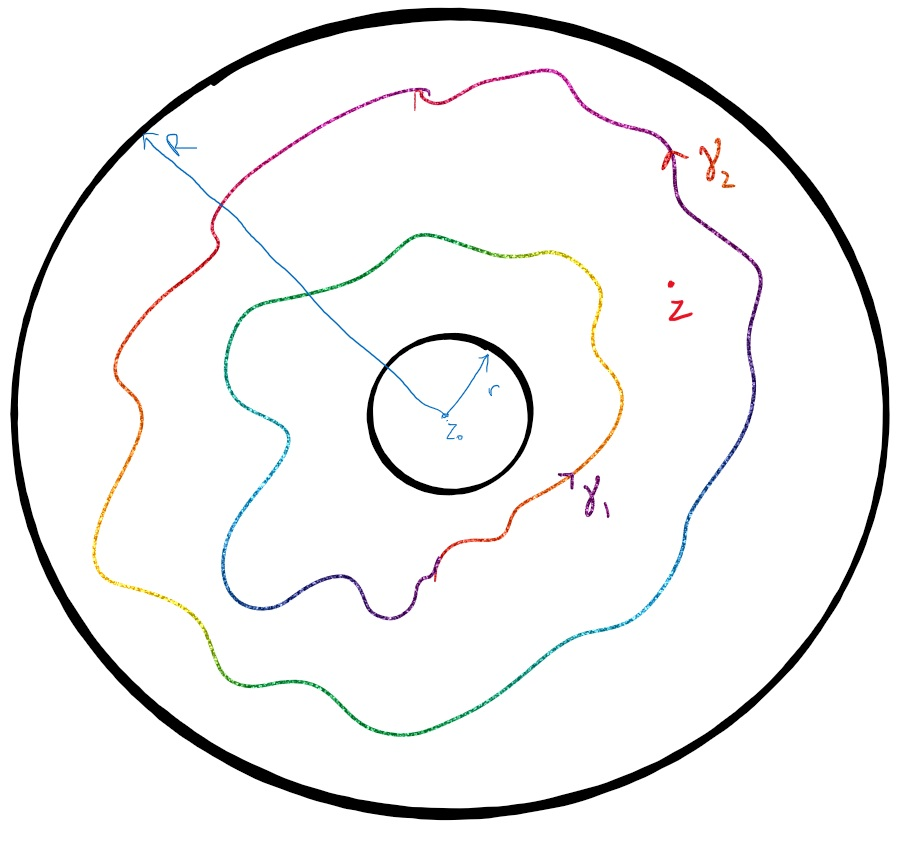
\includegraphics[width=6cm]{CIF-annulus.jpg}
    \end{center}
    \vspace{-2mm}
    \begin{equation*} 
        f(z) = \frac{1}{2 \pi \iota}\left(\int_{\gamma_{2}} - \int_{\gamma_{1}}\right)\frac{f(w)}{w - z} {\mathrm{d}}w.
    \end{equation*}
\end{frame}
\begin{frame}{Lecture 9: Laurent Series}
    \begin{thm}[Laurent Series]
        With the same setup as earlier, for $z \in A,$ we can write $f(z)$ as\uncover<2->{
        \begin{equation*} 
            f(z) = \sum_{n = -\infty}^{\infty}a_n(z - z_0)^n,
        \end{equation*} }\uncover<3->{where each $a_n$ is given, as before, by }\uncover<4->{
        \begin{equation*} 
            a_n = \dfrac{1}{2\pi\iota}\int_{|w - z_0| = r_0}^{} \dfrac{f(w)}{(w - z_0)^{n + 1}} {\mathrm{d}}w,
        \end{equation*} }\uncover<5->{where $r < r_0 < R.$ } 
    \end{thm}
    \uncover<6->{Note that the above is valid for $n < 0$ as well. }
\end{frame}
\begin{frame}{Lecture 9: Laurent Series}
   \begin{defn}[Laurent series expansion at $z_0$]
        If $z_0$ is an isolated singularity of $f,$ then $f$ is holomorphic in an annulus $\{z : 0 < |z - z_0| < r\}$ for some $r > 0.$ The Laurent series expansion on this annulus is called the Laurent series expansion \textbf{at} $z_0.$ 
   \end{defn}
   \begin{defn}[Principal part]
       Let $\displaystyle\sum_{n = -\infty}^{\infty}a_n(z - z_0)^n$ be the Laurent series expansion \emph{at} $z_0.$ Its principal part is 
       \begin{equation*} 
           \displaystyle\sum_{n = -\infty}^{-1}a_n(z - z_0)^n.
       \end{equation*}
   \end{defn}
\end{frame}
\begin{frame}{Lecture 9: Laurent Series}
    The most interesting coefficient of the principal part is the $-1^{\text{st}}$ one. \uncover<2->{When we integrate a Laurent series along a circle centered at $z_0$ (which contains no other singularity), only $a_{-1}$ remains (with a factor of $2\pi\iota$). }\uncover<3->{This is given by
    \begin{equation*} 
        a_{-1} = \dfrac{1}{2\pi\iota}\int_{|z - z_0| = r_0}^{} f(w) {\mathrm{d}}w.
    \end{equation*} }\uncover<4->{This is what is usually called the \emph{residue} and written as }\uncover<5->{
    \begin{equation*} 
        a_{-1} = \operatorname{Res}(f; z_0).
    \end{equation*} }
\end{frame}
\begin{frame}{Lecture 9: Laurent Series}
    With residues, calculation of integrals becomes easier.
    \begin{thm}[Cauchy's Residue Theorem]
        Suppose $f$ is given and has finitely many singularities $z_1, \ldots, z_n$ within a {\color{red}simple} closed contour $\gamma.$\uncover<2->{Then, we have
        \begin{equation*} 
            \int_{\gamma}^{} f(z) {\mathrm{d}}z = 2\pi\iota\sum_{i = 1}^{n}\operatorname{Res}(f; z_i).
        \end{equation*} }
    \end{thm}
    \uncover<3->{Note that the above is implicitly implying that $f$ is holomorphic at all other points within $\gamma.$ }
\end{frame}
\begin{frame}{Lecture 9: Laurent Series}
    Recall that given an isolated singularity, we can expand the function as a Laurent series \emph{around} that point on a punctured neighbourhood. \uncover<2->{We had defined the principal part of this series to be the part containing the negative powers of $z - z_0.$ We now see how they are related to the nature of the isolated singularity. }
    \begin{thm}[Isolated singularities and their principal parts]
        \uncover<3->{The isolated singularity $z_0$ is }
        \begin{enumerate}
            \uncover<4->{\item removable iff the principal part has no terms, }
            \uncover<5->{\item a pole iff the principal part has finitely many (and at least one) terms, and }
            \uncover<6->{\item essential iff the principal part has infinitely many terms. }
        \end{enumerate}
    \end{thm}
    \uncover<7->{In particular, the residue at a removable singularity is $0.$ }
\end{frame}
\begin{frame}{Lecture 9: Laurent Series}
    Now, we see how one can calculate residue at a pole. \\
    \uncover<2->{By the previous theorem, we know that $f$ can be written as }\uncover<3->{
    \begin{equation*} 
        f(z) = \dfrac{a_{-m}}{(z - z_0)^m} + \cdots + \dfrac{a_{-1}}{z - z_0} + a_0 + a_1(z - z_0) + \cdots,
    \end{equation*} }\uncover<4->{for some integer $m > 0.$ }\\
    \uncover<5->{Thus,
    \begin{equation*} 
        g(z) = (z - z_0)^mf(z)
    \end{equation*} is holomorphic at $z_0$ (after redefining; note that $z_0$ is a removable singularity for $g$) and }\uncover<6->{ 
    \begin{equation*} 
        a_{-1} = \dfrac{1}{(m - 1)!}g^{(m - 1)}(z_0).
    \end{equation*}}
\end{frame}
\begin{frame}{Lecture 10}
    \begin{defn}[Neighbourhood of $\infty$]
        A neighbourhood of $\infty$ is a set of the form
        \uncover<2->{
        \begin{equation*} 
            A(0, R, \infty) \vcentcolon= \{z \in \mathbb{C} : |z| > R\}
        \end{equation*} }
        \uncover<3->{for some $R > 0.$ }
    \end{defn}
    \begin{defn}[Isolated singularity at $\infty$]
        \uncover<4->{$f$ is said to have an isolated singularity at $\infty$ if }\uncover<5->{$f$ is (defined and) holomorphic on some neighbourhood of $\infty.$ }\uncover<6->{Equivalently, $z\mapsto f\left(\dfrac{1}{z}\right)$ has an isolated singularity at $0.$ }  
    \end{defn}
\end{frame}
\begin{frame}{Lecture 10}
    \begin{defn}[Nature of isolated singularity at $\infty$]
        The nature of the singularity of $f$ at $\infty$ is defined to be \uncover<2->{the nature of the singularity of $z \mapsto f\left(\dfrac{1}{z}\right)$ at $0.$ }
    \end{defn}
    \uncover<3->{\textbf{Examples.} }
    \begin{enumerate}
        \uncover<4->{\item $f(z) = 0$ has a removable singularity at $\infty.$ }
        \uncover<5->{\item $f(z) = \dfrac{1}{z}$ has a removable singularity at $\infty.$ }
        \uncover<6->{\item $f(z) = z^n$ has a pole of order $n$ at $\infty.$ ($n \in \mathbb{N}.$) }
        \uncover<7->{\item $\exp$ has an essential singularity at $\infty.$ }
    \end{enumerate}
    \uncover<8->{We didn't define the residue at $\infty.$ Check Wikipedia for what the definition is, if interested. It is not the same as the residue of $f(1/z)$ at $0.$ }
\end{frame}
\begin{frame}{Lecture 11}  
    \begin{thm}[Maximum Modulus Theorem]
        \uncover<2->{Let $\Omega$ be a {\color{red}domain}. }\uncover<3->{Let $f:\Omega\to\mathbb{C}$ be holomorphic }\uncover<4->{and non-constant. }\uncover<5->{Then, $|f|$ does not attain a maximum. }
    \end{thm}
    \uncover<6->{Said differently: If $f:\Omega\to\mathbb{C}$ is holomorphic and $|f|$ attains a maximum, then $f$ is constant. }\\
    \uncover<7->{An ``application:'' Suppose that $f$ is defined on the closed unit disc such that it is continuous on the closed disc and holomorphic on the open disc. }\uncover<8->{Since the closed disc is closed and bounded and $f$ is continuous, $|f|$ must attain a maximum on the closed disc. }\uncover<9->{By MMT, this maximum must be on the boundary. }
\end{frame}
\begin{frame}{End of Lectures 10 and 11}
    \begin{tcolorbox}
        Any questions?
    \end{tcolorbox}
\end{frame}
\begin{frame}{Lecture 12}
    \begin{thm}[Schwarz Lemma]
        \uncover<2->{Let $\mathbb{D} = \{z \in \mathbb{C} : |z| < 1\}$ be the open unit disc. }\\
        \uncover<3->{Let $f:\mathbb{D} \to \mathbb{C}$ be holomorphic such that }\uncover<4->{
        \begin{equation*} 
            f(0) = 0 \quad\text{and}\quad |f(z)| \le 1,
        \end{equation*} for $z \in \mathbb{D}.$ }\\~\\
        %
        \uncover<5->{Then, $|f(z)| \le |z|$ for all $z \in \mathbb{D}$ }\uncover<6->{and $|f'(0)| \le 1.$ }\\~\\
        %
        \uncover<7->{Moreover, if $|f(z)| = |z|$ for some $z \in \mathbb{D} \setminus \{0\}$ }\uncover<8->{\emph{or} if $|f'(0)| = 1,$ then }\uncover<9->{$f(z) = \lambda z$ for some $\lambda \in \mathbb{C}$ such that $|\lambda| = 1.$ }
    \end{thm}
\end{frame}
\begin{frame}{Lecture 12}
    \begin{defn}[Open maps]
        \uncover<2->{A function $f:\Omega \to \mathbb{C}$ is said to be an open map if }\uncover<3->{$f(U)$ is open for any open subset $U \subset \Omega.$ }
    \end{defn}
    \begin{thm}[Open Mapping Theorem]
        \uncover<4->{Let $\Omega$ be open and $f:\Omega\to\mathbb{C}$ be {\color{red}non-constant} and holomorphic. }\uncover<5->{Then, $f$ is an open map. }
    \end{thm}
    \uncover<6->{In particular, $f(\Omega)$ is open. }\uncover<7->{As a corollary, if $f:\Omega\to\mathbb{C}$ is holomorphic such that $f(\Omega)$ is not open, }\uncover<8->{then $f$ is constant. }
\end{frame}
\begin{frame}{Lecture 13}
    \begin{thm}[Argument principle]
        \uncover<2->{Let $f$ be a meromorphic on $\Omega.$ }\uncover<3->{That is, the only singularities of $f$ in $\Omega$ are poles.}

        \uncover<4->{Let $\gamma$ be a simple closed curve in $\Omega,$ }\uncover<5->{oriented positively. }\uncover<6->{Moreover, assume that $f$ has no zero or pole along $\gamma.$ Then, }\uncover<7->{
        \begin{equation*} 
            \dfrac{1}{2\pi\iota}\int_{\gamma}^{} \dfrac{f'(z)}{f(z)} {\mathrm{d}}z = N_\gamma(f) - P_\gamma(f),
        \end{equation*} }\uncover<8->{where $N_\gamma(f)$ \uncover<9->{{\color{blue}(resp., $P_\gamma(f)$)}} denotes the number of zeroes \uncover<9->{{\color{blue}(resp., poles)}} of $f$ within $\gamma$ counted with multiplicity \uncover<9->{{\color{blue}(resp., order)}}.  }
    \end{thm}
\end{frame}
\begin{frame}{Lecture 13}
    \begin{thm}[Rouch\'{e}'s Theorem]
        \uncover<2->{Let $f, g:\Omega\to\mathbb{C}$ be holomorphic. }\uncover<3->{Let $\gamma$ be closed curve in $\Omega.$ }\uncover<4->{Suppose that
        \begin{equation*} 
            |f(z) - g(z)| < |f(z)|,
        \end{equation*} }\uncover<5->{for all $z$ on the image of $\gamma.$ }\\~\\
        %
        \uncover<6->{Then,
        \begin{equation*} 
            N_\gamma(f) = N_\gamma(g).
        \end{equation*} }
    \end{thm}
    \uncover<7->{As before, note that the zeroes are counted with multiplicity. For example, $z^{43}$ has $43$ zeroes within the curve $|z| = 1.$ }
\end{frame}
\begin{frame}{Lecture 13}
    \begin{thm}[Existence of harmonic conjugates]
        \uncover<2->{Let $\Omega \subset \mathbb{R}^2$ be a simply connected domain. }\uncover<3->{Let $u:\Omega\to\mathbb{R}$ be harmonic. }\uncover<4->{Then, $u$ admits a harmonic conjugate on $\Omega.$ }\uncover<5->{Moreover, this conjugate is unique, up to an additive constant. }
    \end{thm}
    \uncover<6->{As a corollary, we had gotten that harmonic functions are infinitely differentiable since open discs are simply connected. }
\end{frame}
\begin{frame}{Lecture 13}
    \begin{thm}[Mean Value Property]
        \uncover<2->{Let $w \in \mathbb{R}^2$ and $u$ be a function harmonic on $B_R(w)$ for some $R > 0.$ }\uncover<3->{Let $0 < r < R.$ Then, we have }\uncover<4->{
        \begin{equation*} 
            u(w) = \dfrac{1}{2\pi}\int_{0}^{2\pi} u(w + re^{\iota\theta}) {\mathrm{d}}\theta.
        \end{equation*} }
    \end{thm}
    \uncover<5->{Note that in CIF, we had a $z$ in the denominator. No such thing here. Moreover, we have $2\pi$ instead of $2\pi\iota.$ }\uncover<6->{The latter is of course expected since everything is $\mathbb{R}$eal. }
\end{frame}
\begin{frame}{Lecture 13}
    \uncover<1->{As a corollary, we obtain MMT for harmonic functions which says that $u$ cannot obtain a maximum at any interior point unless it is constant. }

    \uncover<2->{Note that here, we are talking about $u$ directly. }\uncover<3->{\emph{Not} $|u|.$ }\uncover<4->{Applying MMT to $-u$ also gives us that $u$ cannot attain a minimum at any interior point unless it is constant. }

    \uncover<4->{\begin{thm}[Identity Principle for harmonic functions]
        \uncover<5->{Let $u$ be a harmonic function on a domain $\Omega \subset \mathbb{C}.$ }\uncover<6->{If $u = 0$ on a non-empty open subset $U \subset \Omega,$ }\uncover<7->{then $u = 0$ throughout $\Omega.$ }
    \end{thm} }
\end{frame}
\begin{frame}{End of Lectures 12 and 13}
    \begin{tcolorbox}
        Any questions?
    \end{tcolorbox}
\end{frame}
\begin{frame}{Little Picard Theorem}
    \begin{thm}[Little Picard]
        \uncover<2->{Let $f$ be an entire function, }\uncover<3->{i.e., $f:\mathbb{C}\to\mathbb{C}$ is a holomorphic function. }\uncover<4->{If $f$ is nonconstant, then the image of $f$ is either all of $\mathbb{C}$ or $\mathbb{C}$ minus a point. }\\~\\
        \uncover<5->{In other words, if an entire function misses two points, then it must be constant. }
    \end{thm}
\end{frame}
\begin{frame}{Integration theorems}
    \begin{thm}[Jordan's Lemma]
        \uncover<2->{Let $f, g$ be continuous complex valued functions defined on the upper semicircular contour $C_R = \{Re^{\iota\theta} : \theta \in [0, \pi]\}$ for some $R > 0.$ }\uncover<3->{Assume that there exists $a > 0$ such that }\uncover<4->{
        \begin{equation*} 
            f(z) = e^{\iota az}g(z),
        \end{equation*} }\uncover<5->{for all $z \in C_R.$ }\uncover<6->{Then, 
        \begin{equation*} 
            \left|\int_{C_R}^{} f(z) {\mathrm{d}}z\right| \le \dfrac{\pi}{a}\max_{\theta\in[0, \pi]}\left|g(Re^{\iota\theta})\right|.
        \end{equation*}}
    \end{thm}
    \uncover<7->{This is useful in the cases that the quantity on the right goes to $0$ in the limit $R \to \infty.$ }
\end{frame}
\begin{frame}{Integration theorems}
    \begin{thm}[Fractional residue theorem]
        \uncover<2->{Let $f$ have a simple pole at $z_0.$ }\uncover<3->{Fix $\alpha \in (0, 2\pi]$ and $\alpha_0 \in [0, 2\pi).$ }\\~\\
        %
        \uncover<4->{For $r > 0,$ define $\gamma_r(\theta) \vcentcolon= z_0 + re^{\iota(\theta + \alpha_0)}$ for $\theta \in [0, \alpha].$ }\uncover<5->{Then, 
        \begin{equation*} 
            \lim_{r\to 0^+}\int_{\gamma_r}^{} f(z) {\mathrm{d}}z = \alpha\iota\Res(f; z_0).
        \end{equation*}}
    \end{thm}
    \uncover<4->{\begin{center}
            \begin{tikzpicture}
                \def\r{3}
                \def\del{1}
                \def\thet{30}
                \def\alph{100}                
                \draw[red, thick, domain=\thet:\thet+\alph, ->-=at 0.5 with label {\tiny $\gamma_r$}] plot ({\r*cos(\x)}, {\r*sin(\x)});
    
                \draw[thin, domain=\thet:\thet+\alph, ->-=at 0.5 with label {\tiny $\alpha$}] plot ({\del*cos(\x)}, {\del*sin(\x)});
    
                \draw[thin, domain=\thet:\thet+\alph, ->-=at 0.5 with label {\tiny $\alpha$}] plot ({\del*cos(\x)}, {\del*sin(\x)});
    
                \draw[blue, thin, domain=0:\thet, ->-=at 0.5 with label {\tiny $\alpha_0$}] plot ({\del*cos(\x)}, {\del*sin(\x)});
    
                \draw[->] (0, 0) -- (0:1.1*\r);
                \draw[dashed] (0, 0) -- (\thet:\r);
                \draw[dashed] (0, 0) -- ({\thet+\alph}:\r);
                \node[] at (-\r/10, 0) {\footnotesize $z_0$};
            \end{tikzpicture}
        \end{center} }
\end{frame}
\begin{frame}{Integration Theorems}
    Not exactly an integration theorem but something we saw in lectures that is helpful in computing integrals of rational functions.

    \begin{thm}   
        \uncover<2->{Let $P(z)/Q(z)$ be a rational function such that }\uncover<3->{$\deg Q(x) \ge \deg P(x) + 2.$ }\uncover<4->{Then, there exist constants $R_0$ and $C$ such that }\uncover<5->{
        \begin{equation*} 
            \left|\dfrac{P(z)}{Q(z)}\right| \le \dfrac{C}{|z|^2},
        \end{equation*} }\uncover<6->{whenever $|z| > R_0.$ }

        \uncover<7->{Thus, if $R > R_0,$ then $\left|\dfrac{P(z)}{Q(z)}\right| \le \dfrac{C}{R^2}$ on a circle of radius $R.$ }
    \end{thm}

    \uncover<8->{Usually, we will be interested in the upper half semi-circle. }\uncover<9->{ML inequality will tell us that the integral over the semicircle goes to $0$ in the limit $R \to \infty.$ }
\end{frame}
\begin{frame}{The End}
    \begin{tcolorbox}
        Doubts?
    \end{tcolorbox}
\end{frame}
\end{document}